\documentclass[11pt]{beamer}
\usetheme{Darmstadt}
\usepackage{graphicx}
\usepackage[portuguese]{babel}
\usepackage{float}
\usepackage{array}
\usepackage{hyperref}
\title{\textbf{Finanças pessoais}}
\author{Isaura Sofia Xavier Cid \\ 63761 - fc63761@alunos.fc.ul.pt \\ TP18 - Licenciatura em Engenharia Informática}
\date{}

\begin{document}

\begin{frame}
\maketitle
\begin{figure}
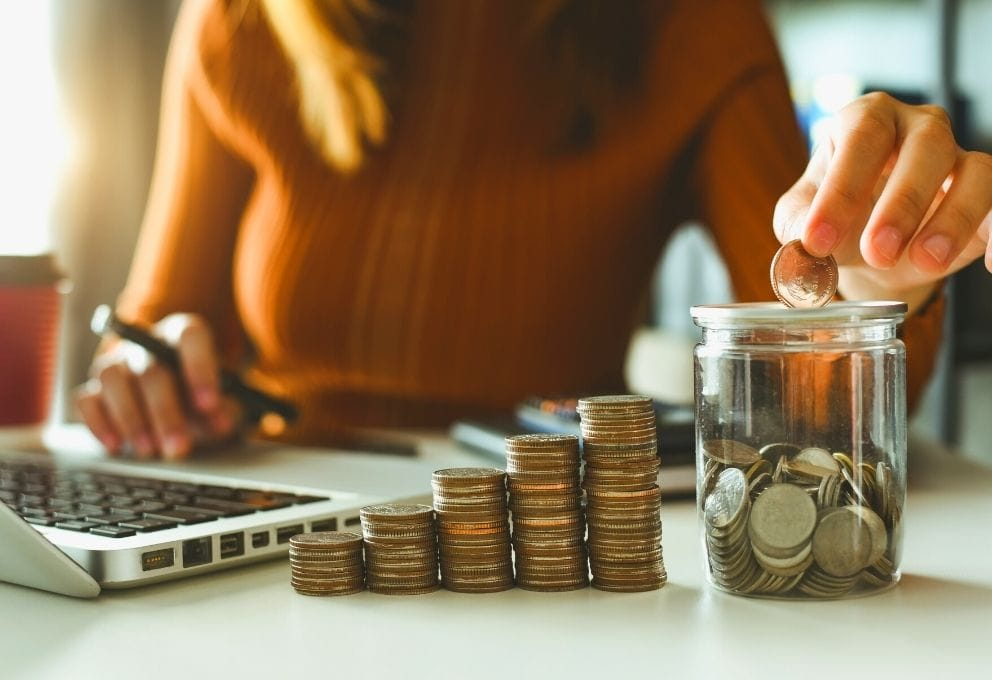
\includegraphics[scale=0.1]{finanças_pessoais.jpg}
\end{figure}
\end{frame}


\begin{frame}{Caso de estudo}
\begin{table}[H]
    \centering
    \caption{Resumo}
    \resizebox{\textwidth}{!}{
    \begin{tabular}{|l|p{2.5cm}|p{2.5cm}|p{2.5cm}|p{2.5cm}|p{2.5cm}|p{2.5cm}|p{2.5cm}|}
    \hline
    RESUMO & Setembro & Outubro & Novembro & Dezembro & Janeiro & Fevereiro & TOTAL \\
    \hline
    RENDIMENTOS &  729,80 € &  729,80 € &  729,80 € &  729,80 € &  729,80 € &  729,80 € & 4 378,80 € \\
    \hline
    GASTOS &  397,83 € &  244,30 € &  232,30 € &  235,30 € &  234,00 € &  214,30 € & 1 558,03 € \\
    \hline
    SALDO DO MÊS &  331,97 € &  485,50 € &  497,50 € &  494,50 € &  495,80 € &  515,50 € & 2 820,77 € \\
    \hline
    SALDO ACUMULADO &  331,97 € &  817,47 € &  1 314,97 € &  1 809,47 € &  2 305,27 € &  2 820,77 € & 9 399,92 € \\
    \hline
    \end{tabular}}
    \label{tabela resumo}
\end{table}
\begin{figure}[H]
\begin{center}
\caption{Rendimentos versus Gastos}
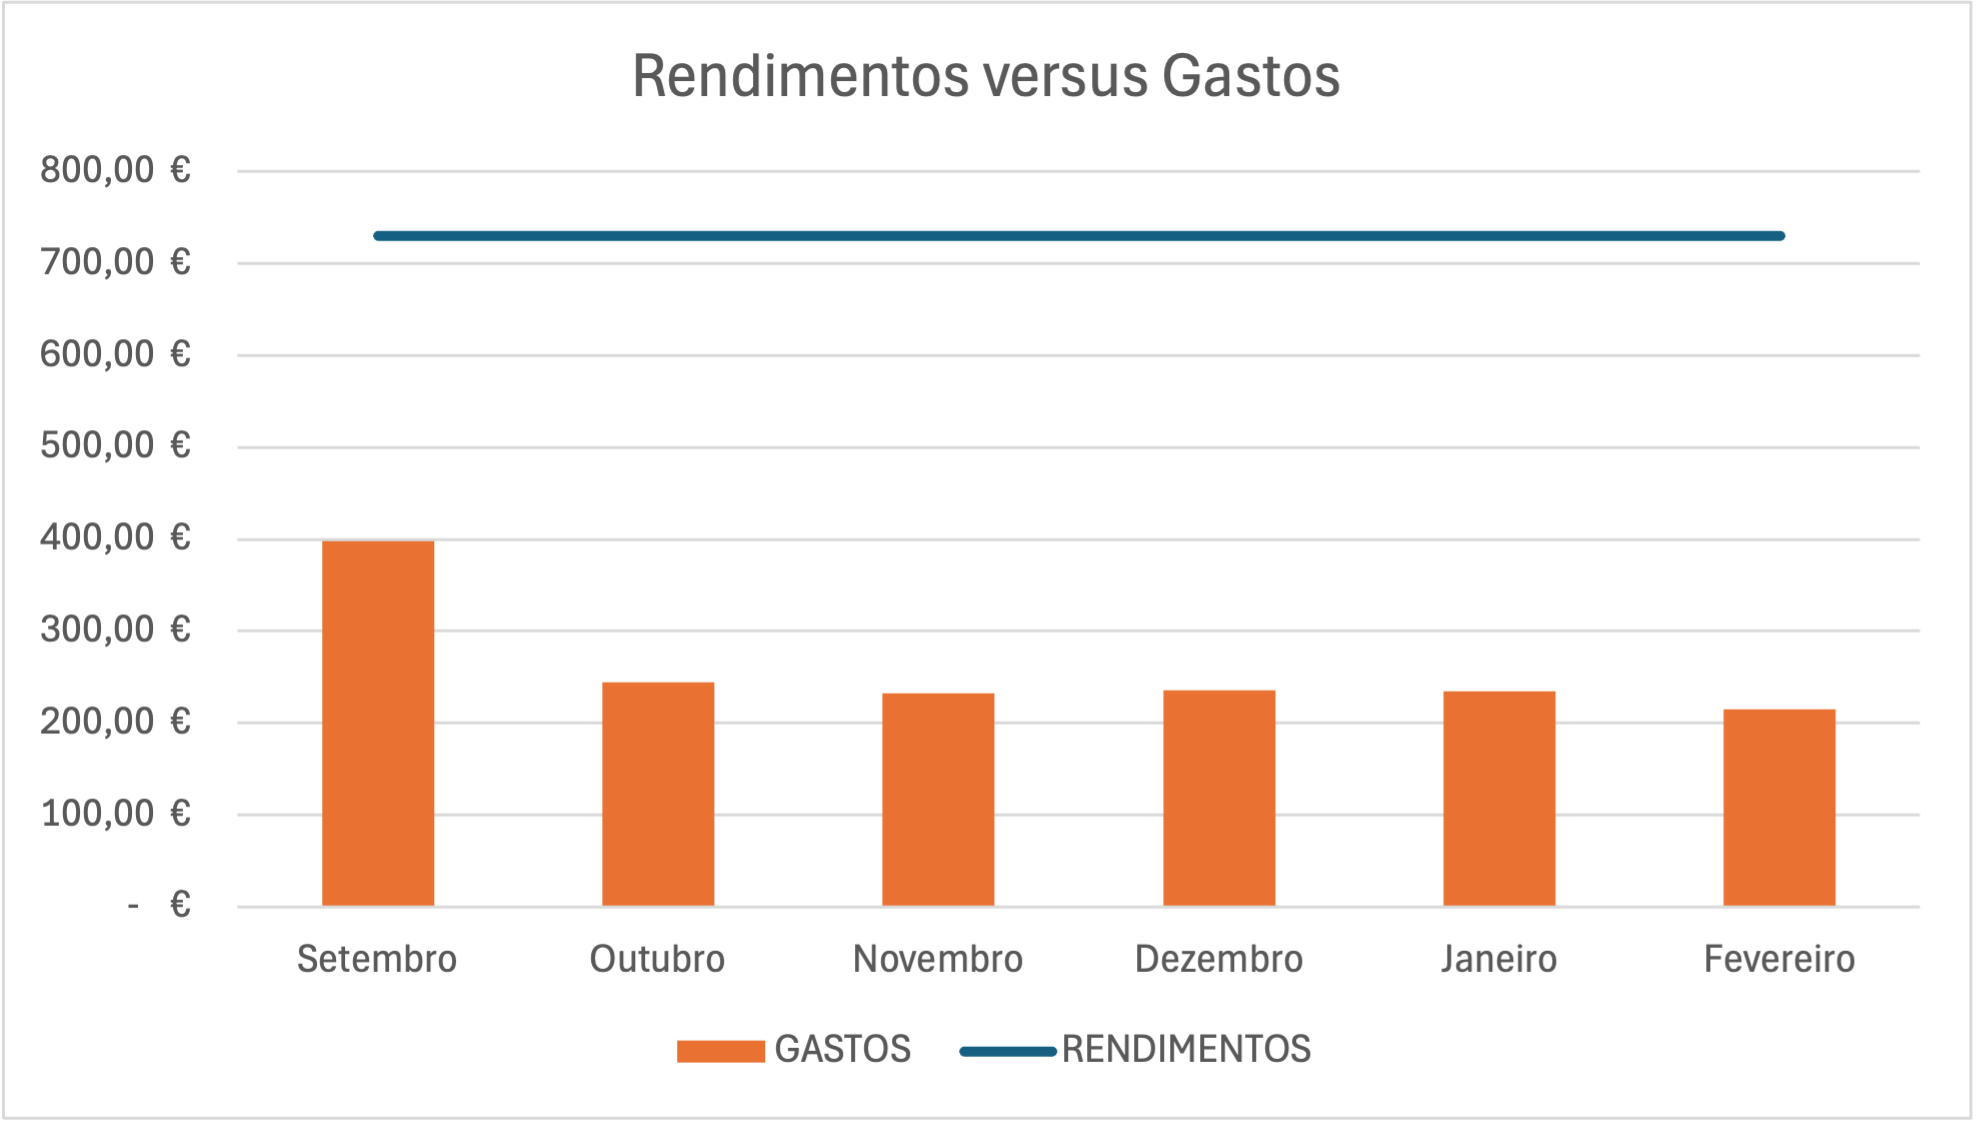
\includegraphics[scale=.3]{gráfico_rendimentosVSgastos.png}
\label{gráfico de barras}
\end{center}
\end{figure}
\end{frame}

\begin{frame}{Caso de estudo}
\begin{table}[H]
    \begin{center}
    \caption{As Contas}
    \scalebox{0.5}{
    \begin{tabular}{|l|l|}
    \hline
        As Contas & TOTAL \\ \hline
        Rendimentos &  4 378,80  €  \\ \hline
        Habitação &  550,80  €  \\ \hline
        Saúde &  30,00  €  \\ \hline
        Transportes &  -    €  \\ \hline
        Despesas Pessoais &  324,23  €  \\ \hline
        Lazer &  80,00  €  \\ \hline
        Ensino &  512,00  €  \\ \hline
        Extras &  61,00  € \\ \hline
    \end{tabular}}
    \label{tabela As Contas}
    \end{center}
\end{table}
\begin{figure}[H]
\begin{center}
\caption{Despesas em percentagem}
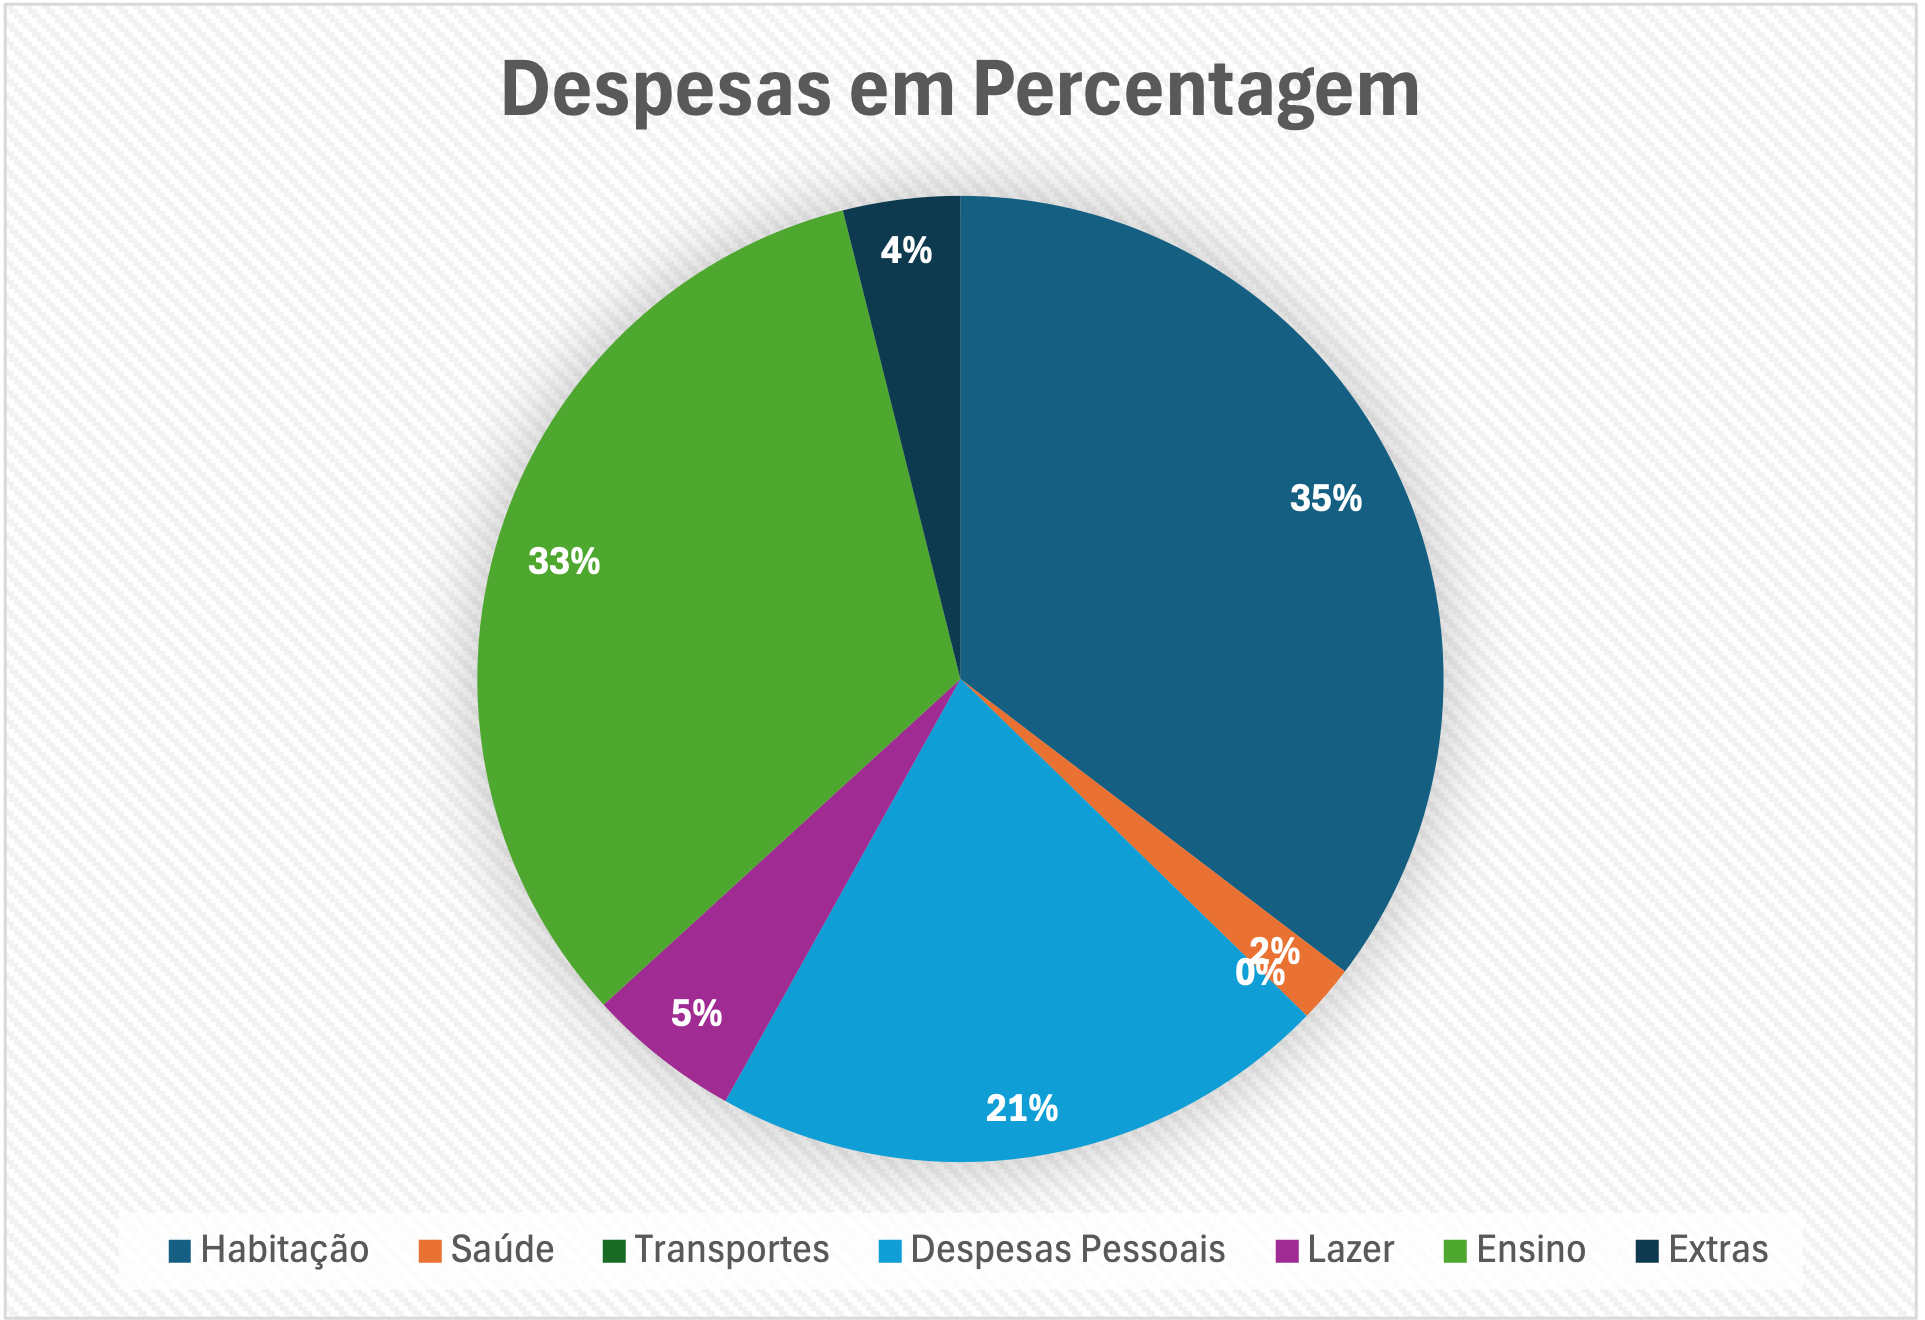
\includegraphics[scale=.3]{despesasEmPercentagem.png}
\label{gráfico circular}
\end{center}
\end{figure}
\end{frame}

\begin{frame}{Modo de preenchimento}
Para preencher os dados da tabela Planeamento:
\begin{itemize}
\item Verifiquei talões 
\item Produtos comprados periodicamente
\begin{itemize}
\item Higiene
\item Medicação
\item etc.
\end{itemize}
\item Produtos essenciais, de acordo com a estação:
\begin{itemize}
\item Em setembro é tempo de comprar o material escolar
\item Em novembro/dezembro é tempo de comprar prendas de natal
\item etc.
\end{itemize}
\end{itemize}
\end{frame}

\begin{frame}{Fim}
\begin{figure}
\begin{center}

\includegraphics[scale=0.5]{financiamento_pessoal}
\end{center}
\end{figure}
Imagem retirada do site: \href{http://www.5docredito.com.br/reestruturacao-financeira/como-organizar-as-financas/}{Reestruturação financeira: como organizar as finanças}
\end{frame}

\end{document}